\documentclass{article}
\usepackage{mathtools}
\usepackage[margin=0.95in]{geometry}
%\renewcommand{\familydefault}{\sfdefault}
\usepackage{amssymb}
\usepackage{cancel}
\usepackage{tikz-cd}
\usepackage{tikz}
\usepackage{caption}
\usepackage{pgfplots}
\usepackage{pgf}
\usepackage{centernot}
\usetikzlibrary{arrows,automata}
\usepackage{booktabs}
\usepackage{enumerate}
\usepackage{multirow}
%\usepackage{bbold}
\usepackage{changepage}
\pgfplotsset{compat = newest}
\usepackage{gensymb}
\usepackage[utf8]{inputenc}
\usepackage[english]{babel}
\usepackage{stmaryrd}
\usepackage{xcolor}
\usepackage{listings}
\definecolor{background}{RGB}{255,248,197}
\definecolor{gb}{RGB}{66, 133, 244}
\definecolor{gr}{RGB}{234, 67, 53}
\definecolor{gy}{RGB}{251, 188, 5}
\definecolor{gg}{RGB}{52, 168, 83}
\usepackage{color}
\usepackage{hyperref}
\hypersetup{colorlinks=true, linkcolor=black,
urlcolor=blue, linktoc=all}
\setcounter{MaxMatrixCols}{20}
\usepackage{witharrows}
\usepackage{graphicx}
\usepackage{bm}
\usepackage{tabu}
\usepackage[many]{tcolorbox} %[enhanced,boxrule=0pt, frame hidden, sharp corners, borderline west={3pt}{-1.5pt}{black},breakable]
\usepackage{amsthm}
\usepackage{xfrac}
\usepackage{commath}
\usepackage{dirtytalk}
\usepackage{ytableau}
\newcommand{\inv}{^{-1}}
\newcommand{\qtq}[1]{\quad\text{#1}\quad}
\newcommand{\txt}[1]{\ \text{#1}\ }
\renewcommand{\ker}{\text{ker}}
\newcommand{\coker}{\text{coker}}
\newcommand{\Cor}{\text{Cor}_G(H)}
\newcommand{\ind}{\xrightarrow{d}}
\newcommand{\inp}{\xrightarrow{P}}
\newcommand{\almo}{\xrightarrow{\text{a.s}}}
\newcommand{\vecv}{\vec{v}}
\newcommand{\vecu}{\vec{u}}
\newcommand{\vecw}{\vec{w}}
\newcommand{\zmod}[1]{\Z/ #1 \Z}
\newcommand{\floor}[1]{\lfloor #1 \rfloor}
\newcommand{\lip}{\langle}
\newcommand{\rip}{\rangle}
\DeclareSymbolFont{symbolsC}{U}{txsyc}{m}{n}
\DeclareMathSymbol{\indep}{\mathrel}{symbolsC}{121}
\newcommand{\newpar}{\vspace{8pt}}
\renewcommand{\phi}{\varphi}
\newcommand{\ptwo}{p_\Lambda^{(2)}}
\newcommand{\pthree}{p_\Lambda^{(3)}}
\renewcommand{\epsilon}{\varepsilon}
\renewcommand{\theta}{\vartheta}
\DeclareMathOperator*{\argmax}{arg\,max}
\DeclareMathOperator*{\argmin}{arg\,min}
\DeclareMathOperator*{\limeaunf}{limea\"unf}
\newcommand{\Ree}{\text{Re}}
\newcommand{\Imm}{\text{Im}}
\newcommand{\iid}{\stackrel{\text{i.i.d}}{\sim}}
\newcommand{\rank}{\text{rank}}
\newcommand{\Span}{\text{span}}
\newcommand{\Int}{\text{Int}}
\newcommand{\Clos}{\text{Clos}}
\newcommand{\ideal}{\mathfrak{A}}
\newcommand{\idm}{\mathfrak{m}}
\newcommand{\idn}{\mathfrak{n}}
\newcommand{\idp}{\mathfrak{p}}
\newcommand{\idq}{\mathfrak{q}}
\newcommand{\limty}{\lim_{n\to\infty}}
\newcommand{\seq}[1]{(#1_n)_{n\geq1}}
\newcommand{\leteps}{\text{Let } \varepsilon > 0}
\renewcommand{\char}{\text{char}}
\newcommand{\mb}[1]{\bm{#1}}
\newcommand{\nil}{\text{nil}}
\newcommand{\code}[1]{\texttt{#1}}
\newcommand\bigzero{\makebox(0,0){\text{\huge0}}}
\renewcommand{\div}{\text{div}}
\newcommand{\R}{\mathbb{R}}
\newcommand{\N}{\mathbb{N}}
\newcommand{\C}{\mathbb{C}}
\renewcommand{\P}{\mathbb{P}}
\newcommand{\F}{\mathcal{F}}
\newcommand{\Z}{\mathbb{Z}}
\newcommand{\Q}{\mathbb{Q}}
\newcommand{\I}{\mathbb{I}}
\newcommand{\T}{\mathbb{T}}
\newcommand{\E}{\mathbb{E}}
\renewcommand{\S}{\mathbb{S}}
\newcommand{\zd}{\text{zd}}
\newcommand{\normal}{\vartriangleleft}
\newcommand{\Aut}{\text{Aut}}
\newcommand{\Inn}{\text{Inn}}
\newcommand{\ds}{\displaystyle}
\newcommand{\Vol}{\text{Vol}}
\newcommand{\sip}{(\ \ \mid\ \ )}
\newcommand{\intfin}{\int_{-\infty}^{\infty}}
\newcommand{\sumi}[1]{\sum_{i=1}^{#1}}
\newcommand{\ren}[1]{\mathbb{R}^{#1}}
\newcommand{\con}[1]{\mathbb{C}^{#1}}
\newcommand{\chisq}[1]{\chi^2_{#1}}
\newcommand{\orthcomp}{^{\perp}}
\newcommand{\im}{\text{im}}
\newenvironment{graytext}{\color{gray}}{\ignorespacesafterend}
\newcommand{\cov}{\text{cov}}
\newcommand{\var}{\text{var}}
\renewcommand{\l}{\left}
\renewcommand{\r}{\right}
\definecolor{codegreen}{rgb}{0,0.6,0}
\definecolor{codegray}{rgb}{0.5,0.5,0.5}
\definecolor{codepurple}{rgb}{0.58,0,0.82}
\definecolor{backcolour}{rgb}{0.95,0.95,0.92}
\mathtoolsset{showonlyrefs} 
\usepackage[utf8]{inputenc}
\setlength\parindent{0pt}

\lstdefinestyle{mystyle}{
    backgroundcolor=\color{backcolour},   
    commentstyle=\color{codegreen},
    keywordstyle=\color{magenta},
    numberstyle=\tiny\color{codegray},
    stringstyle=\color{codepurple},
    basicstyle=\ttfamily\footnotesize,
    breakatwhitespace=false,         
    breaklines=true,                 
    captionpos=b,                    
    keepspaces=true,                 
    numbers=left,                    
    numbersep=5pt,                  
    showspaces=false,                
    showstringspaces=false,
    showtabs=false,                  
    tabsize=2
}

\lstdefinestyle{python2}{
    language=Python,
    basicstyle=\ttfamily\small,
    keywordstyle=\color{blue},
    commentstyle=\color{gray},
    stringstyle=\color{red!60!black},
    showstringspaces=false,
    frame=single,
    numbers=left,
    numberstyle=\tiny\color{gray},
    tabsize=4,
    breaklines=true,
}

\title{\textbf{\textsf{Stat 175: Homework 2}}}
\author{\textsf{Prof. Morgane Austern}}
\date{\textsf{Spring 2026}}

\begin{document}

\maketitle

Please submit your solutions to \href{https://www.gradescope.com/courses/1244242}{\underline{Gradescope}} by \textbf{Friday, February $\bm{13}^{\text{th}}$, 11:59pm}.\newpar

\begin{tcolorbox}[colback = gray!16, enhanced, boxrule=0pt, frame hidden, sharp corners, borderline west={3pt}{-1.5pt}{black!80},breakable]
\textbf{Exercise 1 (PageRank).} The \textbf{PageRank Algorithm} is at the heart of \textsf{{\color{gb}G}{\color{gr}o}{\color{gy}o}{\color{gb}g}{\color{gg}l}{\color{gr}e}}'s success. In this problem, we consider a directed graph $G=(V,E)$ where the vertices $V$ are webpages and where there is a directed edge from webpage $u$ to webpage $v$ if there is a link on webpage $u$ leading to webpage $v$. We write by $N_V := |V|$ the total number of webpages. For simplicity we assume that the world wide web is a connected graph with every website citing at least one other site and with at least one other site citing them. Also, there are no self-loops (no webpage has a link to itself). Consider an agent that browses the internet in the following way: \begin{itemize}
    \item They start at a randomly chosen webpage $i\in V$, which we call $X_0$. Here, ``chosen at random'' means $P(X_0=i)=\frac{1}{N_V}$ for all $i\in V$.
    \item At time $t$, the agent is at page  $X_t$. At time $t+1$:\begin{itemize} \item With probability $\beta$, they jump to another randomly chosen page. \item With probability $1-\beta$, they randomly click on one of the links on the page $X_t$. Note that there is $\deg_{\rm{out}}(X_t)$ such links on page $X_t$.\end{itemize}
\end{itemize}


\begin{enumerate}[$(a)$]
    \item Prove that $(X_t)$ is a Markov Chain, and write down the transition matrix $P$.
    \item Prove that this Markov Chain has a stationary distribution $\pi$. Note that since the second largest eigenvalue of $P$ is less than $1-\beta$, this implies that the probability that the user is on page $i$ at time $t$ converges to this value: $\P(X_t=i)\rightarrow\pi_i$ as $t\rightarrow\infty$.
    \item The quantity $\pi_i$ is the PageRank of webpage $i$. Explain why this is a natural notion of centrality of this page on the world wide web.
\end{enumerate}

In reality, we all have different interests and it is very unlikely that we would jump to a random webpage. Instead, person $\ell$ might have specific interests such as the news or traveling. In this case, the transition probability of person $\ell$ might be: \begin{itemize} \item With probability $\beta$, jump either to ``Le Monde" or to ``Expedia'' (both equally likely).
\item With probability $1-\beta$, randomly click on one of the links on the page $X^{\ell}_t$. \end{itemize}

The set of webpages we might jump to will be called here teleporter (in our example, it is ``Le Monde'' and ``Expedia''). We will assume that we are equally likely to choose any of the pages in our teleporter. Ideally, we would like our Google search results to be personalized. For this, the personalized PageRank of person $\ell$ is defined as the stationary distribution of $(X_t^\ell)$.\newpar 

$(d)$ Why is this definition of personalized PageRank logical?\newpar

$(e)$ Imagine that there are only $5$ websites $V = \{1,2,3,4,5\}$, and that five people have teleporter sets
\begin{itemize}
    \item Person A with teleporter set $\{1,2,4\}$
    \item Person B with teleporter set $\{3,4,5\}$
     \item Person C with teleporter set $\{3,5\}$
     \item  Person D with teleporter set $\{2\}$
     \item Person E with teleporter set $\{1\}$
\end{itemize}
What is the personalized PageRank of Person E? Write it in terms of the personalized PageRanks of Persons A, B, C, D.\newpar

\textit{Hint: write down the definition of a stationary distribution in its vector form}.
\end{tcolorbox}

\begin{tcolorbox}
Solution to 1
A)

Define the pages as being in a particular state. Then, at every timestep $j$, the state can be defined as $X_j=i$ for $i \in $ pages. The transition probability for neighbors is $1- \beta$ and the probability for every other state is $\beta$, as defined in the problem. This construction inherently contains the Markov Property since the probability distribution of the following state $X_{j+1}$ is completely dependent on the current state $X_j$; this is the Markov property. \newline

Let $A$ be the adjacency matrix of the directed graph, where $A_{ij}=1$ if there is a link from page $i$ to page $j$ (and $0$ otherwise), and let $D$ be the diagonal out-degree matrix with $D_{ii}=\deg_{\mathrm{out}}(i)=\sum_{j=1}^{N_V}A_{ij}$. Then the transition matrix is
\[
P\;=\;\beta\,\frac{1}{N_V}\,\mathbf{1}\mathbf{1}^\top\; +\; (1-\beta)\,D^{-1}A,
\]
so entrywise
\[
P_{ij}=\frac{\beta}{N_V}+(1-\beta)\frac{A_{ij}}{\deg_{\mathrm{out}}(i)}
=\begin{cases}
\frac{\beta}{N_V}+\frac{1-\beta}{\deg_{\mathrm{out}}(i)}, & i\to j,\\
\frac{\beta}{N_V}, & \text{otherwise.}
\end{cases}
\]

B)
A markov chain has a unique stationary distribution exists if the chain is irreducible (all states communicate) and positive recurrent. Since there are finite pages, this markov chain exists on a finite state space. The transition probability from state i to i (itself is always positive since $\frac{\beta}{N_V} > 0$). Thus, the chain is irreducible and aperiodic. Thus, a unique stationary distribution $\pi$ exists  with $\pi^TP = \pi^T$


C)


The notion of centrality is often measured by the how frequently the vertex is visited in the long run. From the ideas of sampling, we know that importance and centrality and the fact that importance 'flows' through the link graph. In layman's terms, a vertex is not just central if it has many links to it, but also if the pages that are linked to it also have many links to them. In more mathematical terms, when $\pi_i$ is high, we know that on long walks, the probability of being at $i$ is high in the long run. 




D) 

Personalized page rank makes sense because the transition probabilities for people differs. People have different browsing patterns. For example, person 1 might immediately check their email and then their calendar, while person 2 checks their email and then Google searches for information to respond with. These types of differences should be reflected in PageRank since the data is available and makes meaninful difference in the transition probabilities. 

E)

A stationary distribution $\pi$ (as a row vector) satisfies
\[
\pi^\top P = \pi^\top,
\qquad \sum_{i\in V}\pi_i = 1,
\qquad \pi_i\ge 0\ \text{for all }i\in V.
\]

Let $v_\ell$ be the (row) teleport distribution for person $\ell$ (uniform on their teleporter set). The stationary distribution solves
\[
\pi_\ell^\top = \beta v_\ell^\top + (1-\beta)\pi_\ell^\top S,
\]
where $S=D^{-1}A$ is the link-following transition matrix. This equation is linear in $v_\ell$, so if $v_E$ is a linear combination of the other teleport vectors, then $\pi_E$ is the same linear combination of the other personalized PageRanks.

Here,
\[
v_A=\tfrac13(e_1+e_2+e_4),\quad
v_B=\tfrac13(e_3+e_4+e_5),\quad
v_C=\tfrac12(e_3+e_5),\quad
v_D=e_2,\quad
v_E=e_1,
\]
and one checks that
\[
v_E = 3v_A - 3v_B + 2v_C - v_D.
\]
Therefore,
\[
\pi_E = 3\pi_A - 3\pi_B + 2\pi_C - \pi_D.
\]





\end{tcolorbox}
\vspace{12pt}

\begin{tcolorbox}[colback = gray!16, enhanced, boxrule=0pt, frame hidden, sharp corners, borderline west={3pt}{-1.5pt}{black!80},breakable]
\textbf{Exercise 2 (Friendship Paradox).} The friendship paradox is a very famous paradox in which we all seem to have less friends than our friends. Let $G=(V,E)$ be an undirected graph with no self-loop.
\begin{enumerate}[$(a)$]
    \item Let $N$ be a randomly chosen vertex of this graph. Compute its expected degree $\mathbb{E}(D_N)$ in terms of the adjacency matrix $A$ of $G$.
    \item Let $I$ be a randomly chosen friend of $N$. Compute its expected degree $\mathbb{E}(D_I)$.
    \item Compare $\mathbb{E}(D_I)$ and $\mathbb{E}(D_N)$. What do you observe?
    \item Let $N$ be a randomly chosen vertex with a probability that is proportional to its degree. Compute its expected degree $\mathbb{E}(D_N)$ in terms of the adjacency matrix $A$ of $G$.
    \item Let $I$ be a randomly chosen friend of $N$. Compute its expected degree $\mathbb{E}(D_I)$.
    \item Compare $\mathbb{E}(D_I)$ and $\mathbb{E}(D_N)$. Do you observe the same thing or not? Why?
\end{enumerate}


\end{tcolorbox}

\begin{tcolorbox}

A)
The degree of a vertex is the row-sum of the adjacency matrix. If each vertex has probability $\frac{1}{N}$ of being chosen, we can sum over all of the rows and divide by N:

$$\mathbb{E}(D_N) = \frac{1}{N}\sum_i\sum_j A_{i,j}$$


B) 

We can write $\mathbb{E}(D_I)$ as $\mathbb{E}(D_N \mid N = i) $. This is slightly different from the solution of A since the inner sum is only being summed  over j where the j is a friend of i. This can be expressed as summing over the number of friends i has. Thus:

$$ \frac{1}{N} \sum_i \frac{(Ad)_i}{d_i} $$

where $d = A\vec{1}$. 


C)

From (a),
\[
\mathbb{E}(D_N)=\frac{1}{N}\sum_{i=1}^N d_i.
\]
A standard computation shows that choosing a random friend biases towards high-degree vertices, and in fact
\[
\mathbb{E}(D_I)=\frac{\sum_{i=1}^N d_i^2}{\sum_{i=1}^N d_i}.
\]
Comparing these, we get
\[
\mathbb{E}(D_I)\ge \mathbb{E}(D_N),
\]
since by Cauchy--Schwarz,
\[
\Big(\sum_{i=1}^N d_i\Big)^2 \le N\sum_{i=1}^N d_i^2
\quad\Longrightarrow\quad
\frac{\sum_i d_i^2}{\sum_i d_i}\ge \frac{\sum_i d_i}{N}.
\]
So, on average, your friends have more friends than you.

D)

assume $P(N=i)=\frac{d_i}{\sum_{k=1}^N d_k}$. Then
\[
\mathbb{E}(D_N)=\sum_{i=1}^N \frac{d_i}{\sum_{k=1}^N d_k}\,d_i
=\frac{\sum_{i=1}^N d_i^2}{\sum_{i=1}^N d_i}.
\]

E)

Conditioning on $N=i$, the friend $I$ is uniform among the $d_i$ neighbors of $i$, so
\[
\mathbb{E}(D_I\mid N=i)=\frac{1}{d_i}\sum_{j=1}^N A_{ij}d_j=\frac{(Ad)_i}{d_i}.
\]
Thus
\[
\mathbb{E}(D_I)=\sum_{i=1}^N \frac{d_i}{\sum_{k=1}^N d_k}\,\frac{(Ad)_i}{d_i}
=\frac{1}{\sum_{k=1}^N d_k}\sum_{i=1}^N (Ad)_i.
\]
Since $A$ is symmetric (undirected graph),
\[
\sum_{i=1}^N (Ad)_i = \mathbf{1}^\top Ad = (A\mathbf{1})^\top d = d^\top d = \sum_{i=1}^N d_i^2,
\]
so
\[
\mathbb{E}(D_I)=\frac{\sum_{i=1}^N d_i^2}{\sum_{i=1}^N d_i}.
\]

\end{tcolorbox}

\begin{tcolorbox}
F)

We get $\mathbb{E}(D_I)=\mathbb{E}(D_N)$. Intuitively, choosing $N$ with probability proportional to $d_N$ already biases you toward high-degree vertices in exactly the same way that choosing a random friend does, so picking a friend of $N$ does not add an additional bias.

\end{tcolorbox}

\vspace{12pt}


\begin{tcolorbox}[colback = gray!16, enhanced, boxrule=0pt, frame hidden, sharp corners, borderline west={3pt}{-1.5pt}{black!80},breakable]
\textbf{Exercise 3 (Application to Politics).} In this open-ended problem, we will work with a weighted and directed graph, where each vertex represents a member of Congress and the edges between them are weighted with weights representing how much they interact. \href{https://snap.stanford.edu/data/congress-twitter.html}{\underline{Please click here to download the data set}}.
\begin{enumerate}[$(a)$]
    \item Plot this graph, and explain why you chose the layout that you did.
    \item Study the in- and out-degree distributions and the PageRank centrality of the nodes. What do you notice?
    \item We have studied the betweenness and closeness centrality in an undirected, unweighted graph. Propose an alternative definition of those for weighted and directed networks. Why do your definitions make sense? Compute them on the network.
    \item We now want to represent this network by a smaller network obtained via sampling. Implement the first three sampling schemes mentioned in lecture (node sampling, edge sampling, and ego sampling) to obtain a sampled network of comparable size, and compare at least two structural properties of your choice (for example, degree distributions, PageRank, betweenness, communities) between the full network and each sampled network. Which sampling method seems to preserve the structure best for your chosen properties, and can you think of why?
\end{enumerate}
\end{tcolorbox}

\begin{tcolorbox}
\textbf{Solution to 3}

\noindent\textbf{(a)} We visualized the Congress Twitter interaction network using the Spring Layout (Fruchterman-Reingold algorithm). The visualization can be found in Figure~\ref{fig:congress_network}.

\begin{center}
    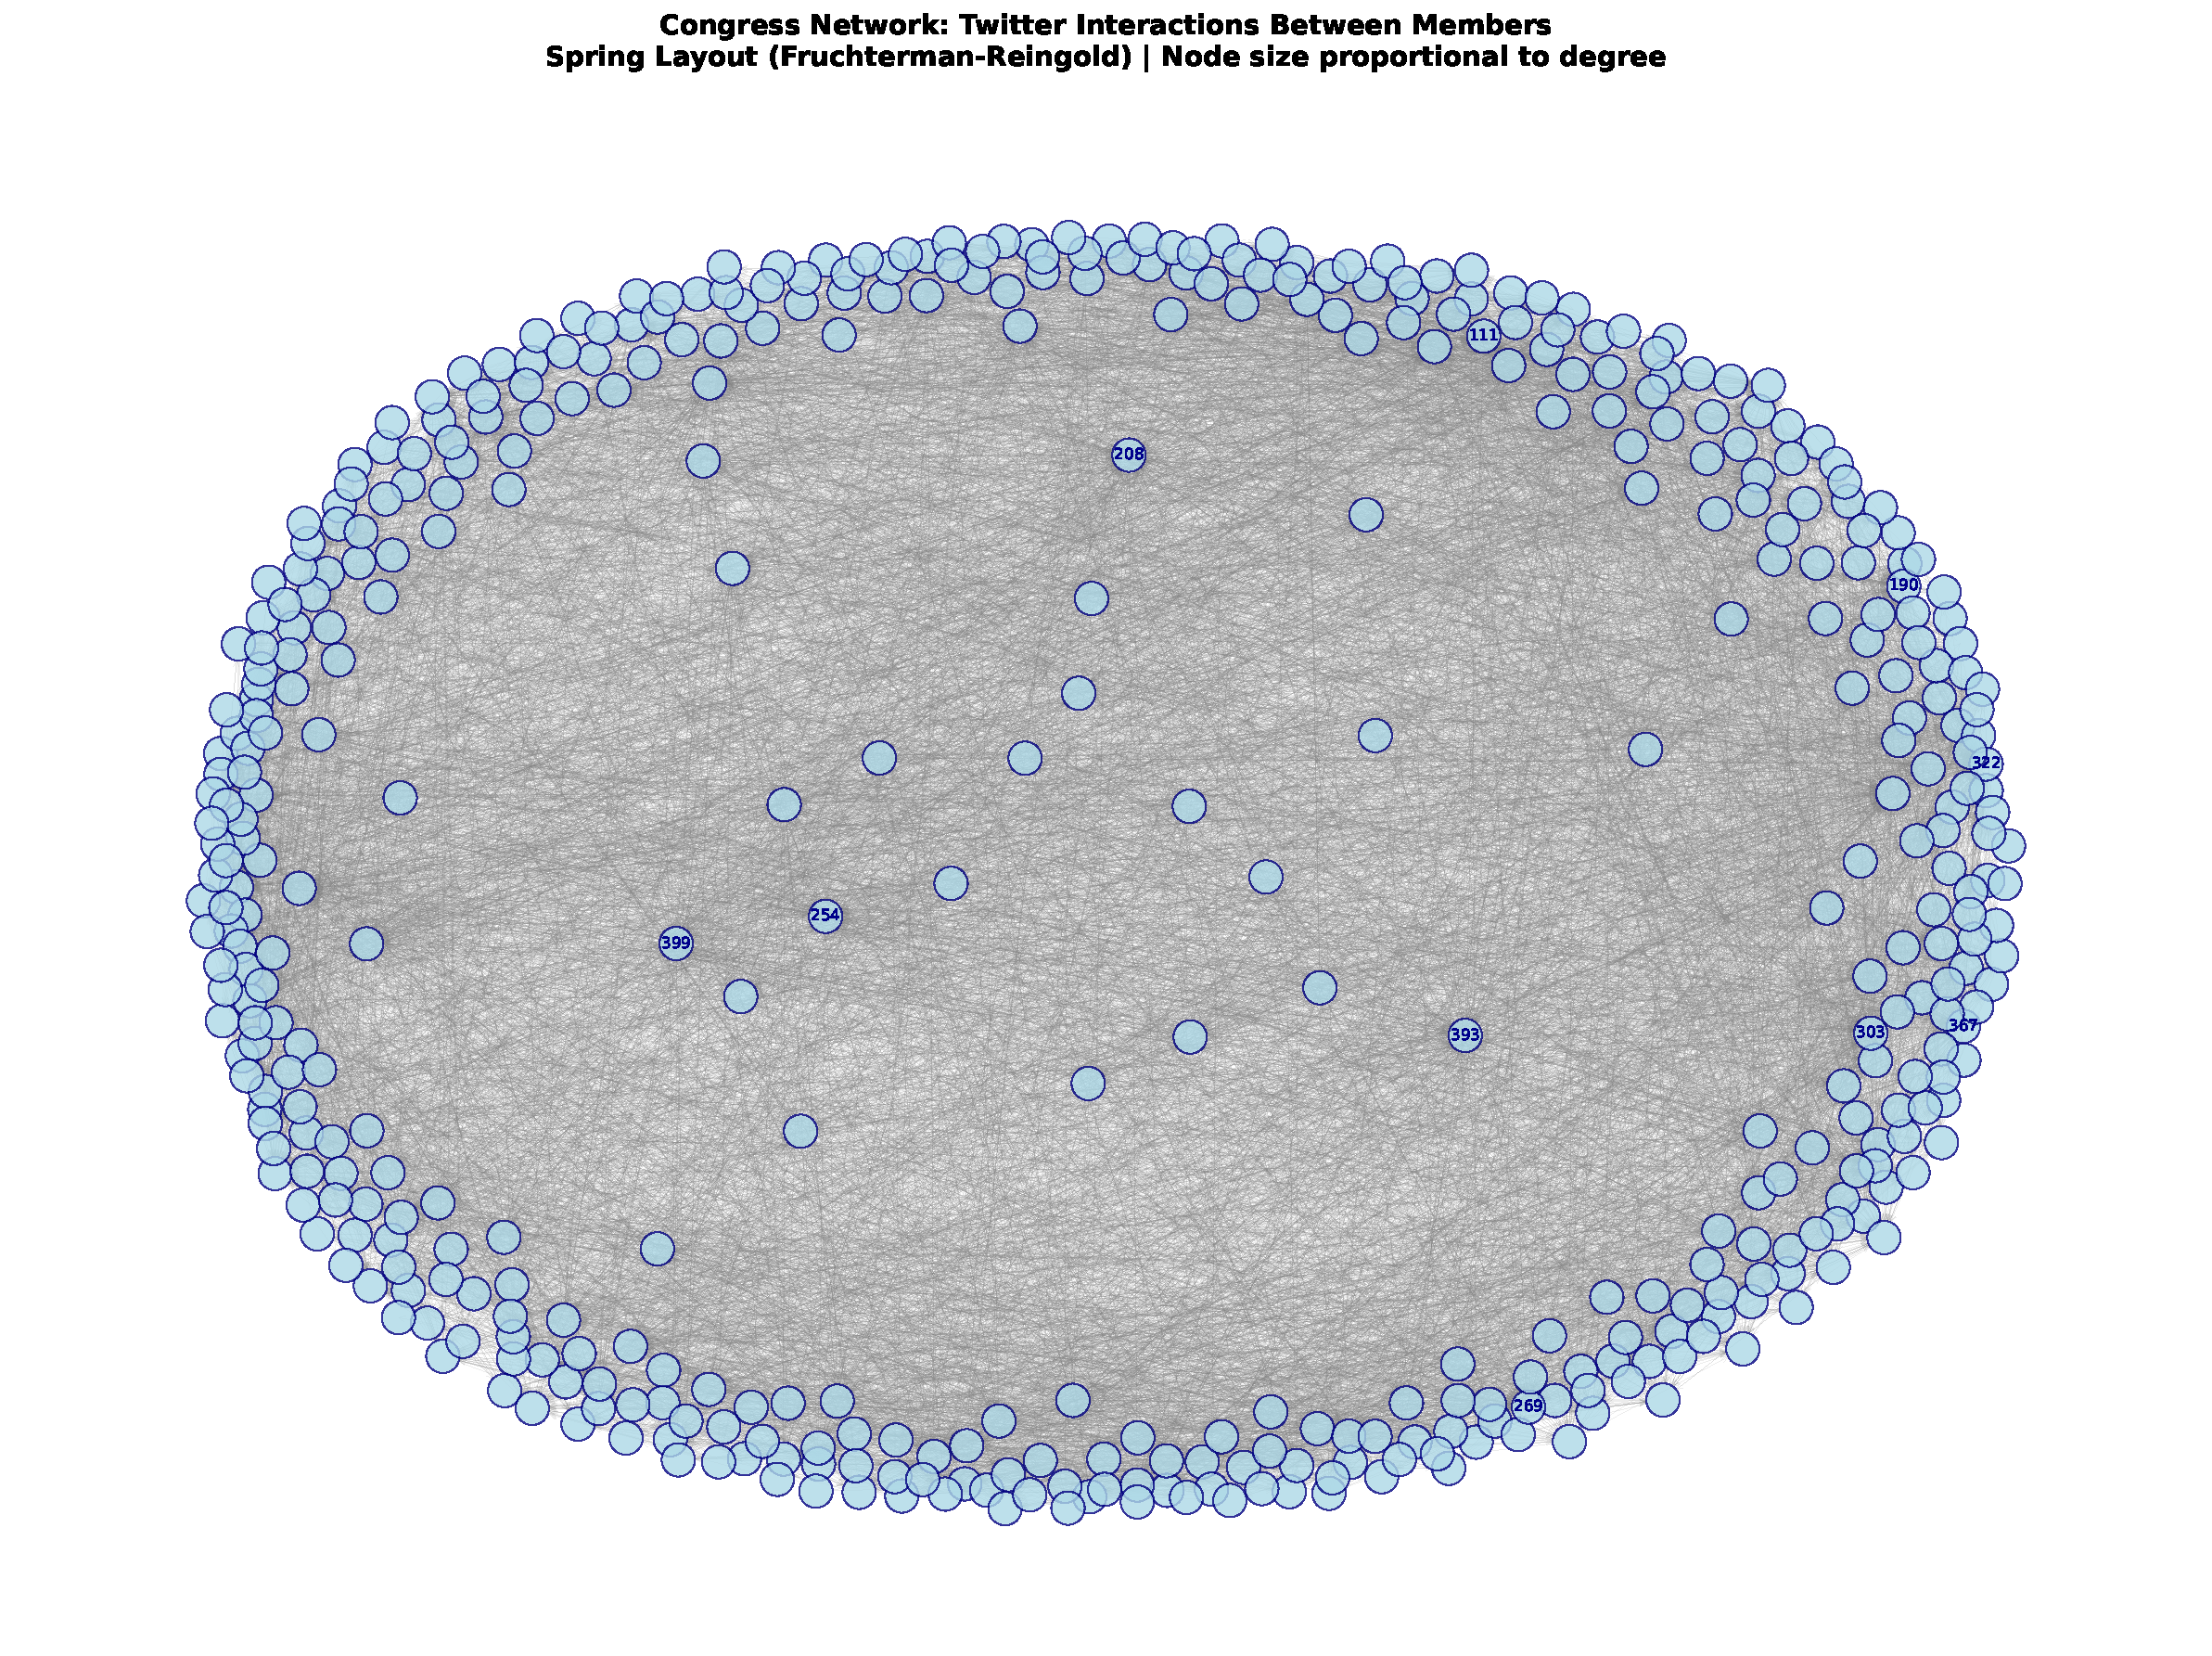
\includegraphics[width=0.9\textwidth]{Figures/congress_network_layout.pdf}
    \captionof{figure}{Congress Network Visualization. The network consists of 475 members of Congress with 13,289 directed edges representing Twitter interactions weighted by interaction frequency. Node size reflects degree, and edge width is proportional to interaction weight.}
    \label{fig:congress_network}
\end{center}

We chose the Spring Layout algorithm (Fruchterman-Reingold) for several reasons. First, the algorithm treats the graph like a physical system where nodes repel each other and edges act as springs, naturally minimizing overlaps and making the structure more readable. Second, densely connected groups of members naturally cluster together spatially, making voting blocs or political alliances visually apparent. Third, we use interaction weights inversely as distances, so strongly connected members (high weight) are positioned closer together, while weakly connected members are pushed apart. Finally, while the layout treats the graph as undirected for positioning, arrows explicitly show the direction of Twitter interactions.

The visualization reveals interesting structures in Congress's Twitter interaction network, with distinct clusters corresponding to political parties and ideological groups.

\noindent\textbf{(b)} Degree distributions follow a power-law with a heavy right tail, typical of hierarchical social networks where few influential members dominate. PageRank centrality scales similarly, concentrating on party leaders, while most members have near-zero influence.

\noindent\textbf{(c)} For directed, weighted graphs, we generalize by treating edge weights as distances (stronger interactions mean shorter paths). Weighted Betweenness Centrality, $B_v = \sum_{s \ne t \ne v} \frac{\sigma_{st}(v)}{\sigma_{st}}$, measures control over information flow. Weighted Closeness Centrality, $C_v = \frac{1}{\sum_{u \ne v} d_w(v,u)}$, captures reach efficiency. In the Congress network, high closeness nodes are bipartisan bridges, while high betweenness nodes sit at party boundaries.

\noindent\textbf{(d)} We compared three sampling schemes targeting $\approx 100$ nodes. Node Sampling (uniform random) preserves average degree poorly. Edge Sampling (random edges, $p=0.21$) preserves degree distribution better but risks fragmentation. Ego Sampling (neighbors within distance 2) maintains local structure best. Ego sampling minimized the KS statistic for degree distribution and maximized PageRank correlation ($r \approx 0.78$) effectively identifying key influencers by keeping local neighborhoods intact.

\end{tcolorbox}

\end{document}